\chapter{Implementación del software\label{sec:Implementacion_soft}}

Una vez finalizado el soporte físico del sistema, será necesario implementar a nivel de software todas las funciones deseadas.

El sistema está compuesto por tres microcontroladores, cada uno de ellos con sus propias características y métodos de programación. Debido a esto, a lo largo de este capítulo se explicará con detenimiento el software utilizado individualmente para ellos así como los distintos entornos de desarrollo (\acrshort{IDE}) necesarios.

Los distintos elementos se presentarán siguiendo el mismo orden que la información que se desea adquirir. Este es:
ADS $\Rightarrow$ Microcontrolador $\Rightarrow$ Interfaz inalámbrica $\Rightarrow$ PC.

\section{Microcontrolador STM32F4\label{Software_micro}}

Debido a la complejidad de los microcontroladores de la familia STM32, los desarrolladores han dedicado su tiempo y esfuerzo en crear herramientas que faciliten su programación. Estas herramientas llamadas \acrshort{IDE} contienen una recopilación de funciones, utilidades y ejemplos que simplifican sensiblemente el proceso de diseño e implementación del software que ejecutará el microcontrolador.

Es tan grande la comunidad de desarrolladores que hay detrás del STM que numerosas empresas han visto como una oportunidad de negocio la creación de un \acrshort{IDE} propietario.

\clearpage

\begin{figure} [h]
    \centering
    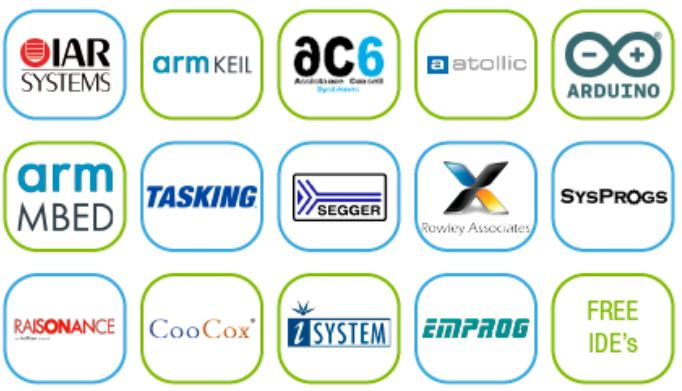
\includegraphics[width=13cm]{STM32_IDEs}
    \caption{IDEs alternativos disponibles \cite{STM32_IDEs}}
    \label{fig:STM32_IDEs}
\end{figure}

La figura \ref{fig:STM32_IDEs} muestra algunos entornos de desarrollo recomendados por el fabricante en su propia página web. Como se puede apreciar, en la imagen se hace distinción entre las opciones comerciales (azul) y las gratuitas (verde).

Uno de los objetivos de este proyecto era utilizar Software Libre en la medida de lo posible. Por ese motivo se probaron algunas de las alternativas presentes en la imagen anterior así como otras menos conocidas basadas en Oracle como ``System Workbench for STM32'' (AC6). A continuación se presentan algunas de las utilizadas al comienzo del proyecto junto con sus características y el motivo de su descarte:
\begin{itemize}
   \item \textbf{CooCox}\\
   Presenta muchos ejemplos prácticos pero su interfaz es muy lenta. Necesita demasiado tiempo para iniciar.
   \item \textbf{Arduino}\\
   Fase muy temprana de desarrollo.
   \item \textbf{System Workbench for STM32}
   \\Buena comunidad pero incompatible con las herramientas de STM.
\end{itemize}

\begin{figure} [h]
    \centering
    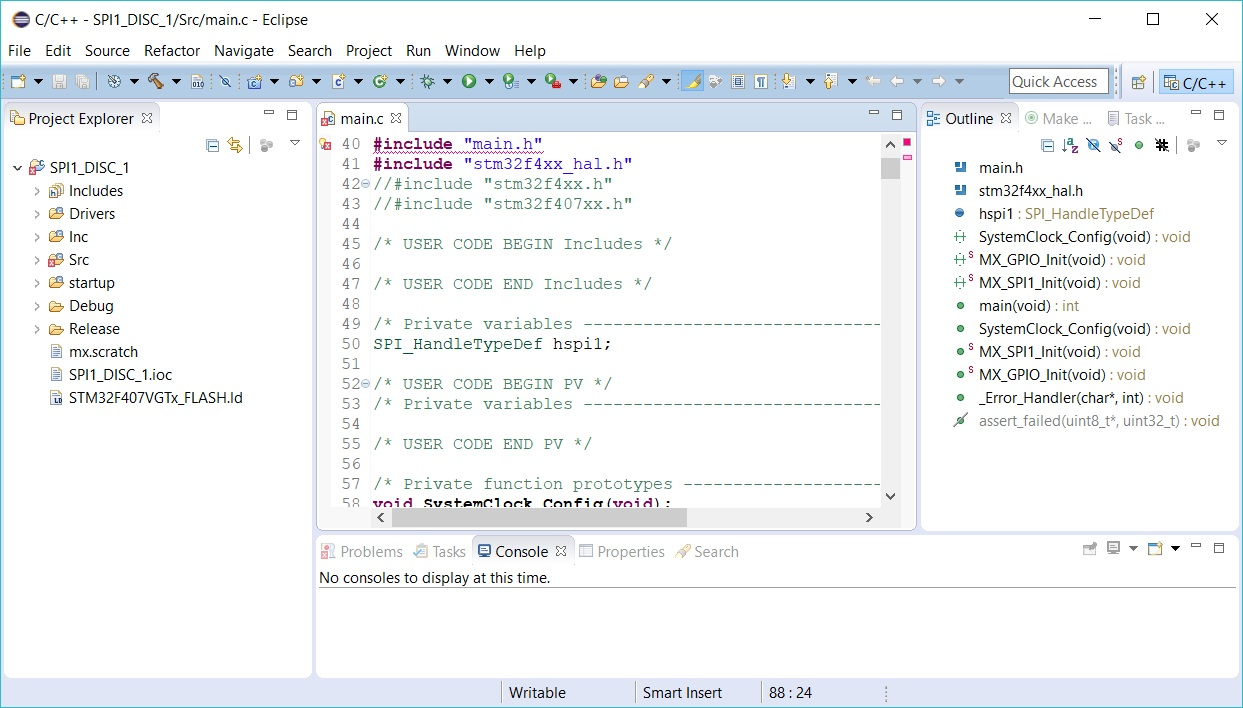
\includegraphics[width=13cm]{Alternative_IDE}
    \caption{Ejemplo de IDE alternativo}
    \label{fig:Alternative_IDE}
\end{figure}

Finalmente se optó por armKeil, pues tiene una gran cantidad de ejemplos y librerías descargables desde la propia interfaz, contiene un gran número de funciones adicionales y la compatibilidad con las herramientas de STM es muy buena. Aunque en la figura \ref{fig:STM32_IDEs} aparece entre las alternativas gratuitas se debe destacar que cuenta con dos versiones, una gratuita que permite realizar proyectos básicos y otra comercial destinada a aplicaciones de mayor envergadura. La limitación de la versión gratuita consiste en forzar un tamaño máximo de programa de 32KB. Si el código a compilar supera dicha longitud directamente no compilará.

\subsection{Configuración inicial\label{Configuracion_micro}}

Aunque Keil permite comenzar un proyecto utilizando como base algunos de los ejemplos que contiene, la configuración de las características del microcontrolador (reloj, interfaces, etc.) puede resultar una tarea muy compleja y tediosa, incluso para aquellos desarrolladores más experimentados. Con el objetivo de facilitar esta tarea, el fabricante ha creado un software con interfaz amigable que permite configurar de forma gráfica el procesador llamado STM32CubeMX.

\begin{figure} [h]
    \centering
    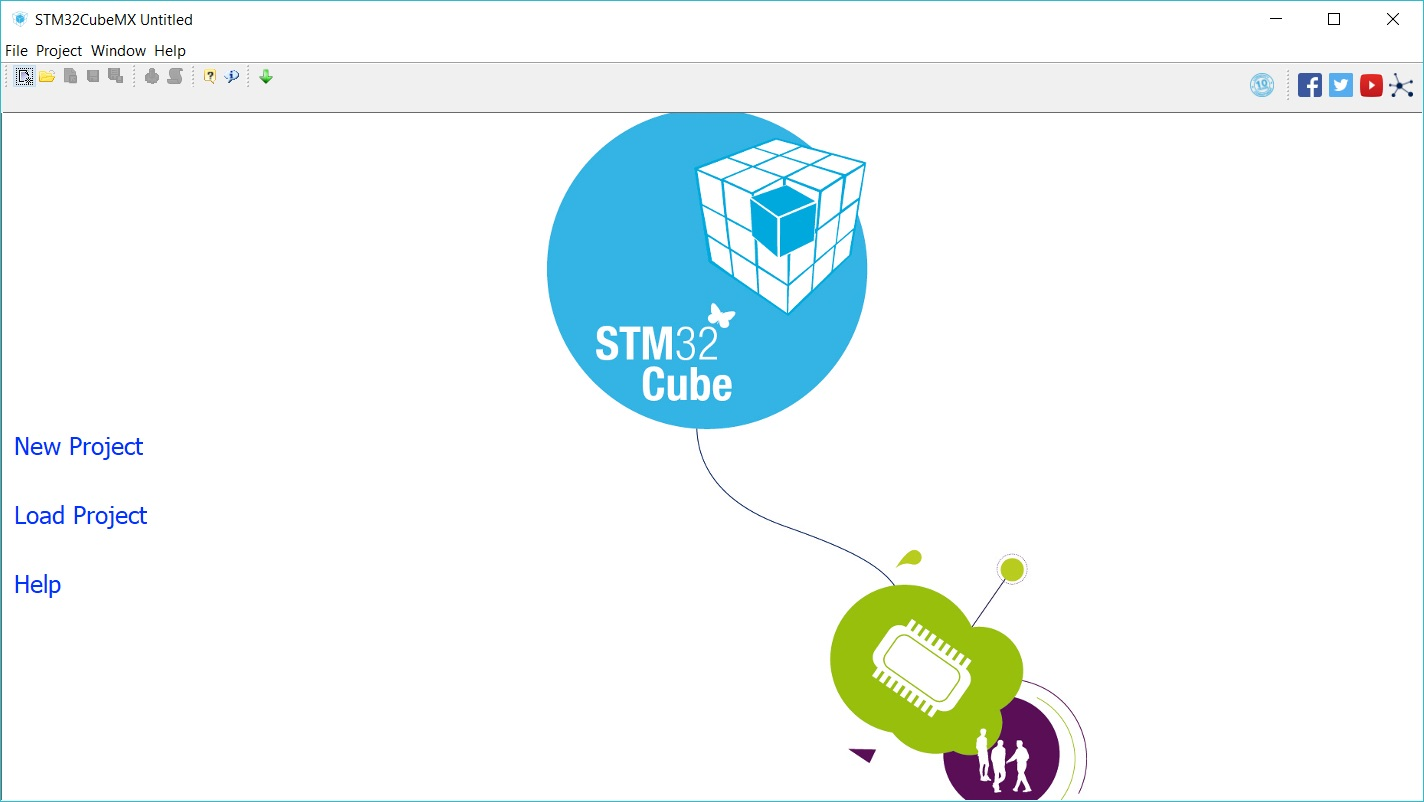
\includegraphics[width=11cm]{STM32CubeMX}
    \caption{Inicializador de proyectos STM32CubeMX}
    \label{fig:STM32CubeMX}
\end{figure}

La herramienta STM32CubeMX incluye una base de datos de todos los microcontroladores disponibles, permitiendo seleccionar el formato, encapsulado e incluso si se va a utilizar en su formato nucleo o en un kit de desarrollo. Incluye también documentación sobre cada microcontrolador y enlaces a distribuidores en caso de que el usuario final quiera comprarlo. 

\subsubsection{Asignación de funciones\label{Configuracion_micro_asignacion}}

Tras seleccionar el microcontrolador, se presenta al usuario una zona de trabajo dividida en cuatro pestañas, cada una destinada a configurar un conjunto de características del microcontrolador: pines y sus funciones, reloj, interfaces de comunicación y consumo de energía.

\begin{figure} [h]
    \centering
    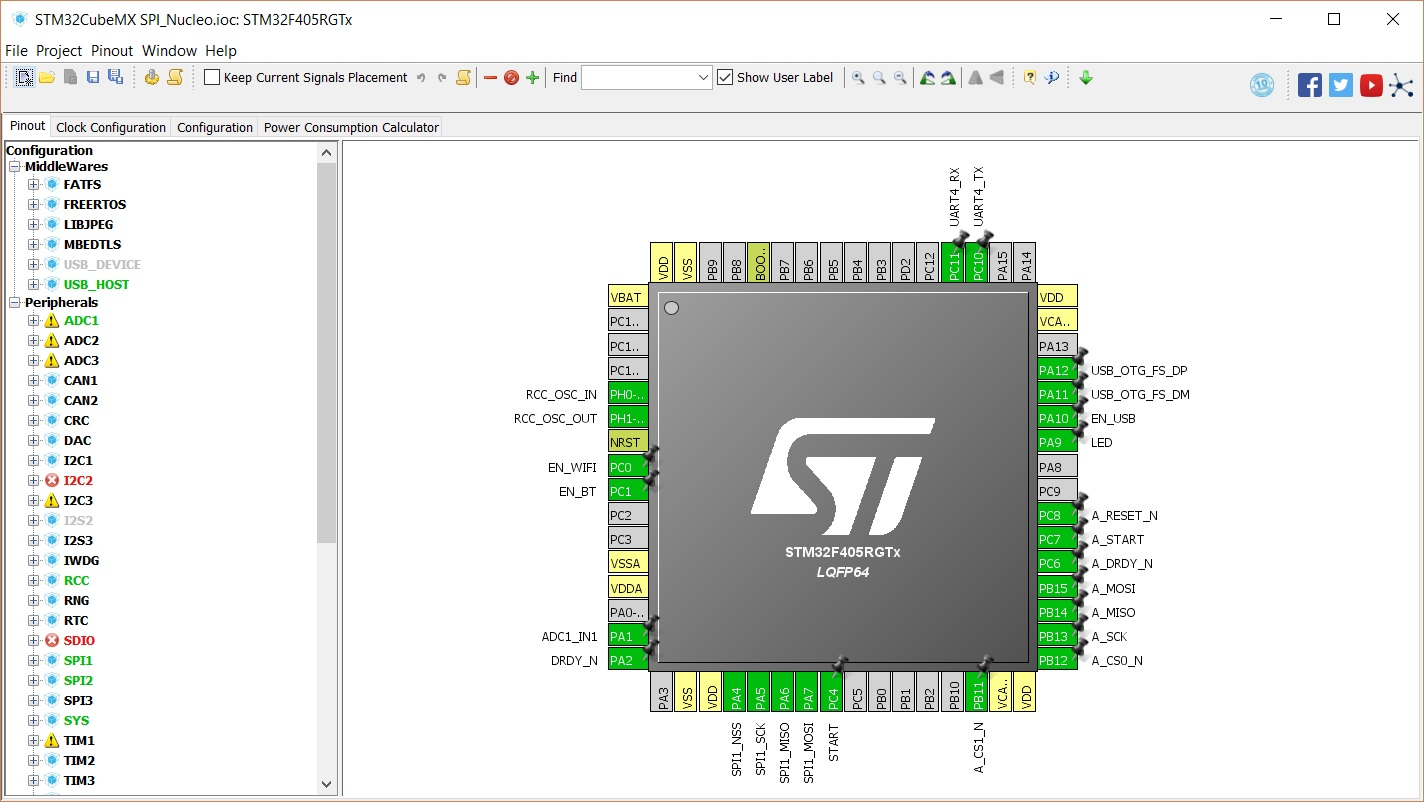
\includegraphics[width=15cm]{STM32CubeMX_pin}
    \caption{Espacio de trabajo del STM32CubeMX}
    \label{fig:STM32CubeMX_pin}
\end{figure}

La configuración de pines permite, no sólo ver de forma visual cada una de las funciones alternativas de cada pin, sino que además indica si alguna no está disponible y las alternativas si se da el caso.

En la figura \ref{fig:STM32CubeMX_pin} aparece la configuración utilizada en este proyecto. En la imagen se puede apreciar que todas las interfaces necesarias para llevar a cabo este proyecto ya han sido asociadas a su pin correspondiente y aún quedan libres casi la mitad de los pines. Esto es un indicador de la versatilidad de este dispositivo.

\subsubsection{Configuración de los relojes\label{Configuracion_micro_reloj}}

Este apartado es el más importante, pues un reloj mal configurado puede provocar errores en la comunicación, una mala gestión del tiempo e incluso que el propio microcontrolador no arranque.

La interfaz desarrollada por STM muestra de forma visual todos los relojes que intervienen en el dispositivo así como las relaciones que hay entre ellos. De esta forma basta con seguir las líneas que conectan los distintos tipos de reloj para saber las dependencias que existen y los resultados que obtendrán en función de los valores escogidos.
\\En caso de que alguna configuración sea incorrecta la propia herramienta está preparada para ofrecer una solución que se acerque lo máximo posible a los resultados deseados.

\begin{figure} [h]
    \centering
    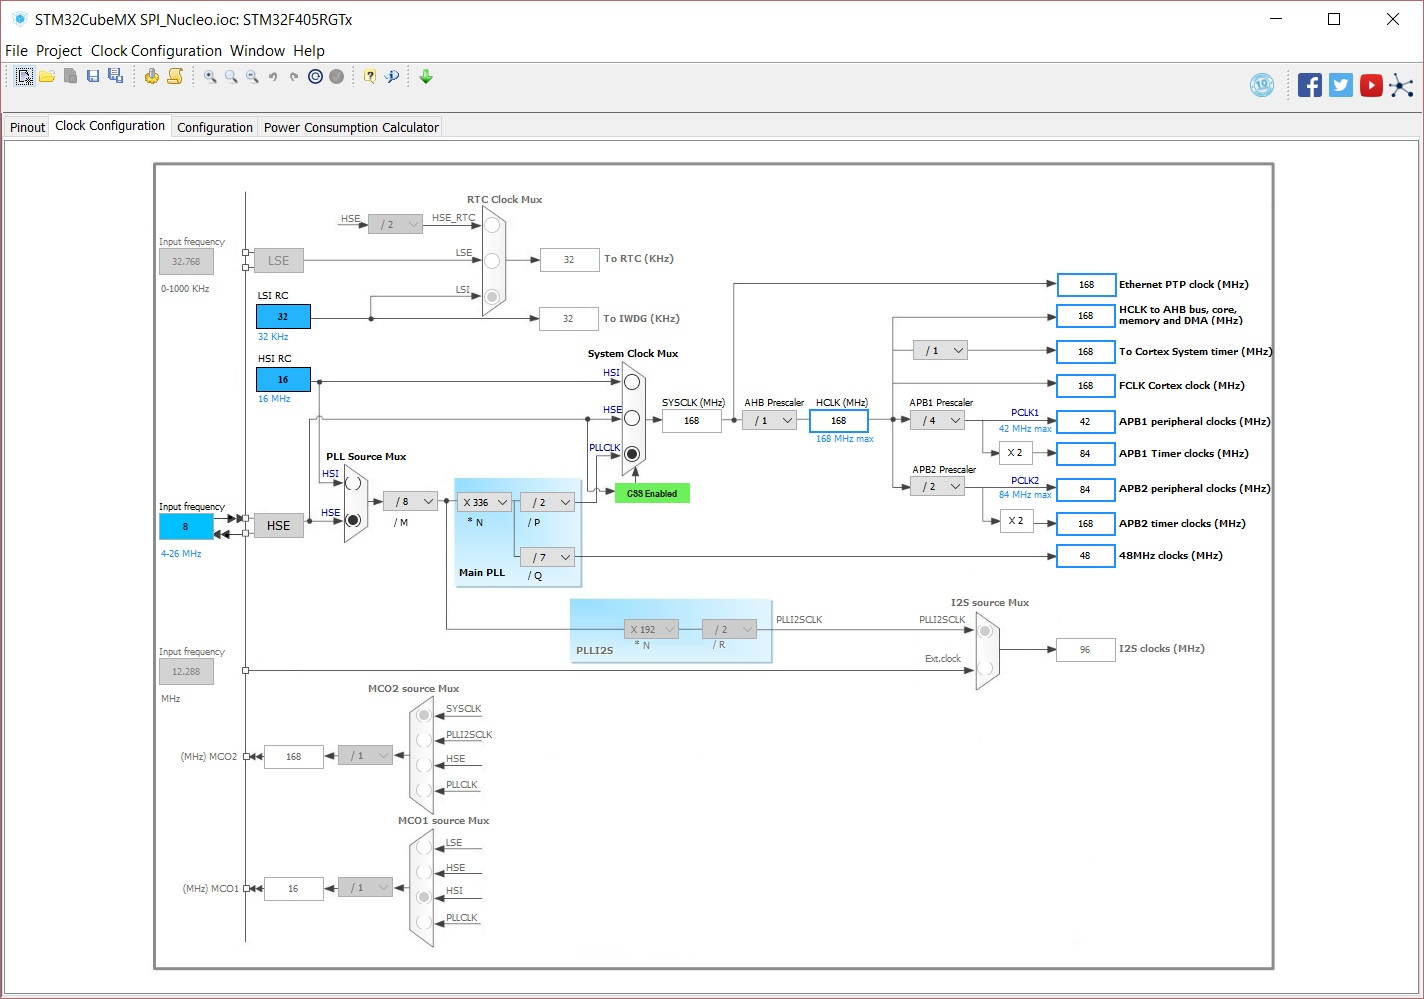
\includegraphics[width=15cm]{STM32CubeMX_clock}
    \caption{Configuración del reloj del microcontrolador}
    \label{fig:STM32CubeMX_clock}
\end{figure}

En la figura \ref{fig:STM32CubeMX_clock} representa la configuración aplicada al microcontrolador durante la realización de este proyecto. A la izquierda se muestran distintas fuentes disponibles mientras que a la derecha se ve la frecuencia final de reloj resultante en cada una de las partes del microcontrolador (periféricos, temporizadores, memoria, etc).

Como se puede ver, aprovecha ambos osciladores, el externo (\acrshort{HSE} = 8MHz) y el interno (\acrshort{LSI} = 16MHz) para, usando \acrshort{PLL}, generar un reloj de una frecuencia mucho más elevada (168 MHz). Dicha frecuencia es, según el fabricante, la máxima frecuencia alcanzable por el dispositivo.

La función \acrshort{CSS} garantiza que, en caso de fallo del reloj del microcontrolador, este generará una alerta y entrará en un modo seguro. Esta función es muy útil cuando se está trabajando con elementos en la seguridad de las personas depende directamente del correcto comportamiento microcontrolador.

\clearpage

\subsubsection{Configuración de los periféricos\label{Configuracion_micro_com}}

La tercera pestaña permite configurar los periféricos, esto incluye interfaces de comunicación, puertos GPIO, USB, etc.

\begin{figure} [h]
    \centering
    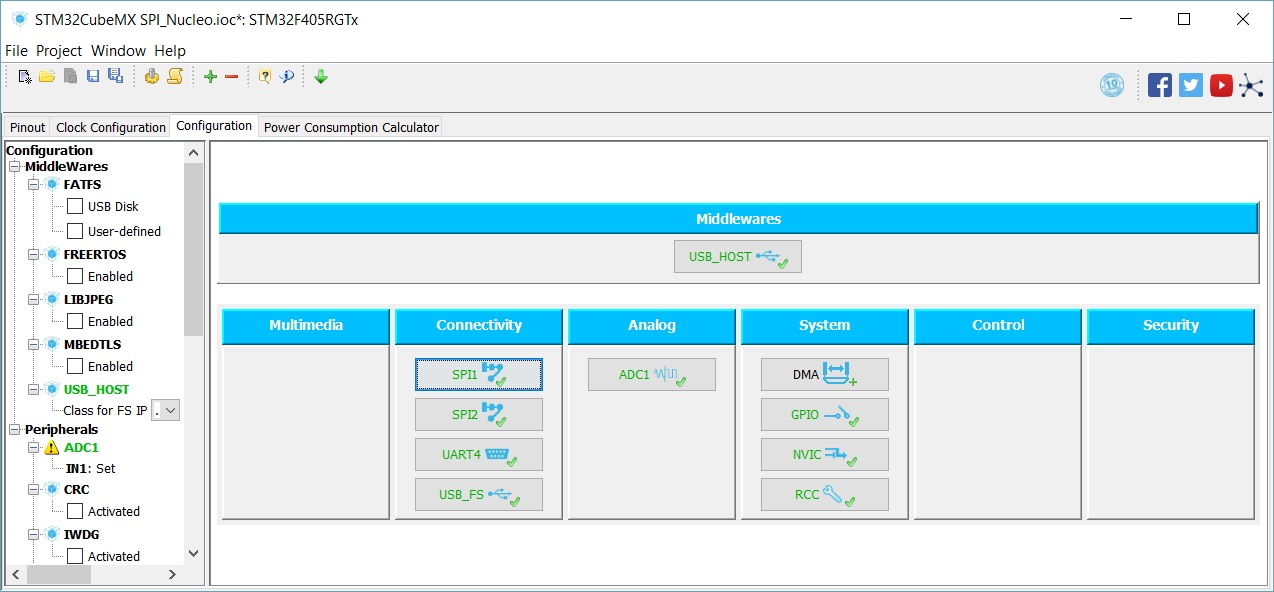
\includegraphics[width=15cm]{STM32CubeMX_conf}
    \caption{Configuración de las interfaces de comunicación}
    \label{fig:STM32CubeMX_conf}
\end{figure}

En función del estado del periférico, este aparecerá marcado con un \textit{tick} verde indicando que todo está correctamente configurado o una cruz roja avisando que alguna característica podría no estar disponible. Además será posible modificar la mayoría de las opciones relacionadas con ese periférico de forma intuitiva. 

\begin{figure} [h]
    \centering
    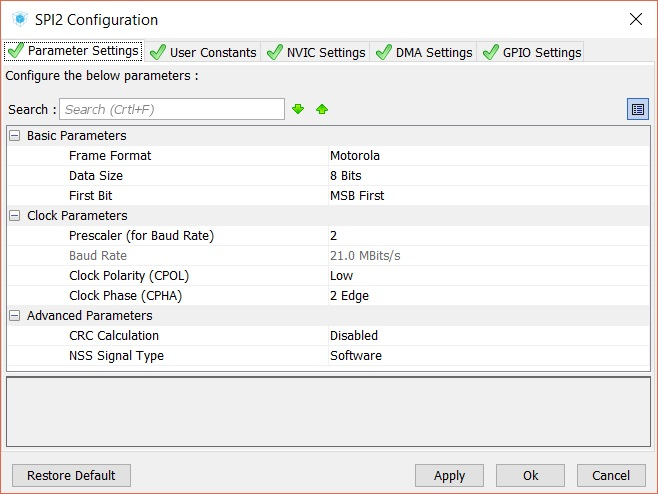
\includegraphics[width=10cm]{STM32CubeMX_conf_2}
    \caption{Detalle de la configuración de las interfaces de comunicación}
    \label{fig:STM32CubeMX_conf_2}
\end{figure}

En la figura \ref{fig:STM32CubeMX_conf_2} se muestran las opciones seleccionadas para el SPI que se comunicará con el los ADS. Se puede cambiar la velocidad, el modo de transmisión e incluso si la gestión del pin ``\textit{Chip-Select}'' se realizará de forma automática o manual.

\subsubsection{Calculo de consumo y otras opciones\label{Configuracion_micro_otro}}

Por último, en la pestaña ``\textit{Power Consuption Calculator}'' mostrada en la figura \ref{fig:STM32CubeMX_otro} se muestran numerosas opciones para el análisis del consumo del microcontrolador en función de parámetros como el modo funcionamiento, la fuente de alimentación e incluso la temperatura.

\begin{figure} [h]
    \centering
    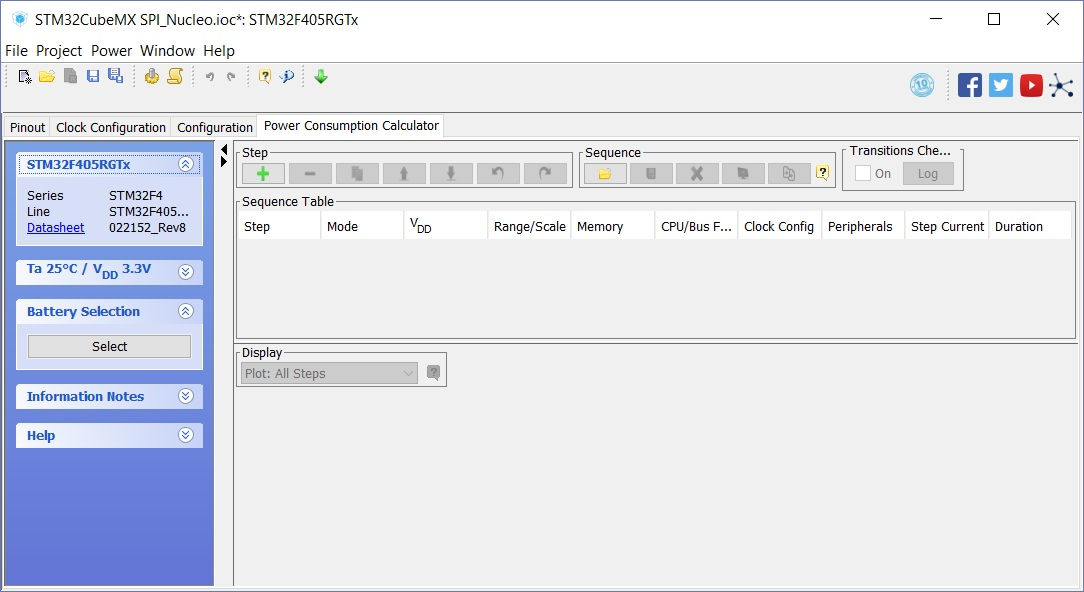
\includegraphics[width=10cm]{STM32CubeMX_otro}
    \caption{Calculadora del consumo del microcontrolador}
    \label{fig:STM32CubeMX_otro}
\end{figure}

Una vez configurado el microcontrolador es necesario seleccionar  activar el generador de código . El STM32CubeMX es capaz de crear un código base para casi cualquier \acrshort{IDE} pero tras un par de usos queda claro que, de entre todos los disponibles, es armKeil con el que la integración da mejores resultados. La herramienta crea el código base con la configuración seleccionada desde la interfaz y lo integra dentro de un proyecto ya configurado y listo para trabajar.

Es importante destacar que la utilización de STM32CubeMX no sólo está pensada para facilitar el comienzo del diseño proporcionando una base sobre la que trabajar, también permite una mayor portabilidad del código ya que, si se siguen las reglas de programación sugeridas por la aplicación, esta permite realizar cambios de la configuración de los pines, los periféricos e incluso de familia de microcontrolador, todo ello sin necesidad de reestructurar el código.

Software
	Comunicación ADS - STM
	
	Comunicación STM- ESP
	
	Arduino (Comunicación ESP - PC)
	
	
